\documentclass[11pt]{article}
\usepackage[utf8]{inputenc}
\usepackage[T1]{fontenc}
\usepackage[spanish]{babel}
\usepackage{graphicx}
\graphicspath{{images/pdf/}{images/jpg/}}

\title{Gobernanza de servicios en la plataforma de interoperabilidad de gobierno electrónico}
\author{Arian Bessonart, Juan Pablo Lucas, Miguel Renom\thanks{Tutores: Laura González, Guzmán Llambías}}
\date{Marzo, 2014}

\begin{document}
	\maketitle
	\pagebreak

	\begin{abstract}
		\emph{Versión preliminar}.
	\end{abstract}
	\pagebreak

	\section{Introducción}
		\subsection{Acerca de la gobernanza en SOA}
			Cuando una organización se plantea la implementación de una arquitectura orientada a servicios (SOA, por sus siglas en Inglés), una de las metas clave en el proyecto es el retorno de inversión positivo. Con el fin de asistir al alcance de dichas metas es que las organizaciones implementan sistemas de gobernanza sobre las arquitecturas.

			La \emph{gobernanza en SOA}, provee las herramientas que asisten a la ejecución de la administración de una SOA, brindando las reglas para la toma de decisiones, estableciendo los procesos necesarios, definiendo los roles que forman parte del sistema administrativo y estableciendo las métricas que determinan el ajuste de la toma de decisiones a las reglas establecidas. La gobernanza no dice cuándo ni cómo tomar una decisión; determina quién debería hacerlo y establece los límites para esa persona o grupo. \cite{Erl:2011:SGG:1983453}

			De entre las varias publicaciones abordando la gobernanza en SOA, en este informe se toma como referencia el \emph{framework} y la terminología propuestas en \cite{Erl:2011:SGG:1983453}.

		\subsection{Proyecto SOA}
			\begin{figure}[h]
			    \centering
			    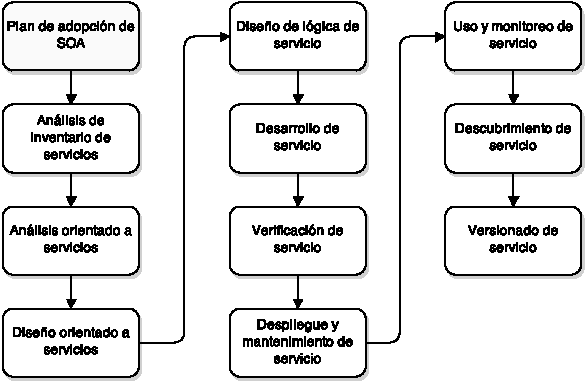
\includegraphics[width=\linewidth]{ciclo_de_vida_del_proyecto}
			    \caption{Etapas comunes de un proyecto SOA}
			    \label{figura:ciclo_de_vida_del_proyecto}
			\end{figure}


			Todo proyecto SOA comienza con un plan de adopción. En este se abordan temáticas tales como el alcance del proyecto (qué servicios), metas, tiempos de ejecución, sistema de gobernanza, forma de financiación, entre otros.

			La figura \ref{figura:ciclo_de_vida_del_proyecto} muestra las etapas comunes de un proyecto SOA las cuales son también etapas del \emph{ciclo de vida} de los servicios.

			En todo proyecto SOA, es de gran importancia el \emph{análisis por adelantado} para la identificación de los servicios. Un servicio pobremente analizado terminará por afectar las metas de la organización en cuanto a la SOA, especialmente en el aporte de valor y retorno de inversión a causa de este último.

			El \emph{análisis de inventarios de servicios} tiene el cometido de definir «blueprints» o planos (cianotipos), los cuales describen las características de un conjunto de servicios pertenecientes a dicho inventario.

			\begin{quote}
				``Un inventario representa una colección de servicios independientemente estandarizados y gobernados''. \cite{Erl:2011:SGG:1983453}
			\end{quote}

			Retomando aquí la importancia del análisis, un mayor esfuerzo en el análisis por adelantado lleva a un cianotipo de inventario de servicios mejor definido, el cual está destinado a la creación de servicios de mayor calidad. Un menor esfuerzo por adelantado lleva a cianotipos parcial o pobremente definidos. \cite{Erl:2011:SGG:1983453}

			En un caso ideal, los inventarios están relacionados directamente con algún \emph{dominio} o línea de negocios de la organización; estos dominios —cuando son más de uno— están a cargo de un propietario dentro de la organización, quien los gobierna. En grandes proyectos, la cantidad de dominios y propietarios —y la relación existente entre ellos— puede resultar propicia para establecer una jerarquía de gobernanza de servicios que permita establecer criterios de adecuados para cada dominio, y a la vez, alineados con los objetivos generales de gobernanza del proyecto SOA. Para ello, el framework deriva la responsabilidad sobre un dominio a la \emph{oficina del programa de gobernanza en SOA} (SGPO, por sus siglas en Inglés).


			Una SGPO es un área encargada de uno o más dominios de servicios dentro de la organización. En una organización dada, múltiples SGPO pueden coexistir en base a los dominios identificados y sus propietarios. En el cuadro \ref{tabla:modelos_sgpo} se listan los diferentes modelos de jurisdicción de SGPO que se pueden aplicar a una organización.

			\begin{table}[h]
				\begin{tabular}{p{0.25\linewidth} | p{0.75\linewidth}}
					\textbf{Tipo} & \textbf{Descripción} \\
					\hline
					SGPO empresarial centralizada & Única SGPO encargada de un único dominio de servicios de la organización\\
					\hline
					SGPO con dominios centralizados & Distintos dominios estandarizados son abarcados por un único sistema de gobernanza dirigido por una SGPO central.\\
					\hline
					SGPO con dominios federados & Varias SGPO responsables de un dominio cada una donde llevan a cabo su propio sistema de gobernanza, el cual debe cumplir con lineamientos introducidos por una SGPO central\\
					\hline
					SGPO con dominios independientes & SGPO individuales responsables de un dominio cada una donde aplican el sistema de gobernanza en forma independiente.\\
					\hline
				\end{tabular}
				\caption{Modelos de jurisdicción de SGPO}
			    \label{tabla:modelos_sgpo}
			\end{table}

			\begin{figure}[h]
			    \centering
			    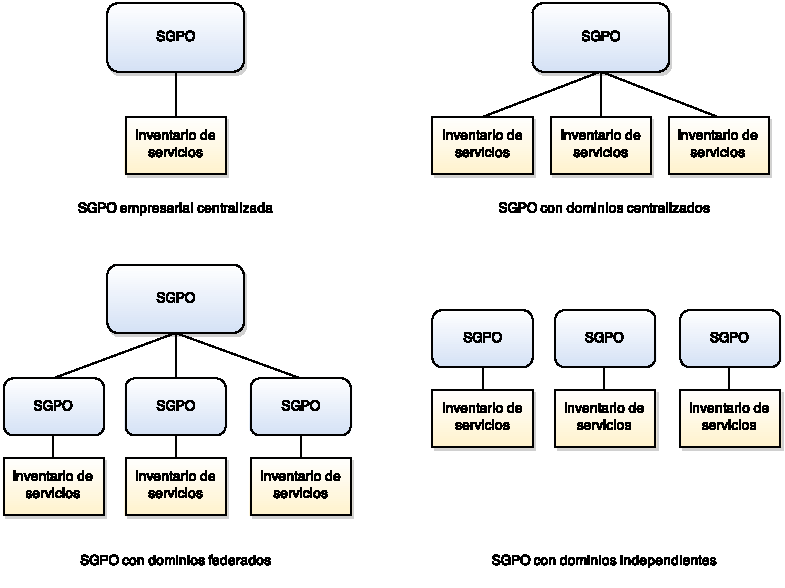
\includegraphics[width=\linewidth]{modelos_sgpo}
			    \caption{Representación gráfica de modelos de jurisdicción de SGPO}
			    \label{imagen:modelos_sgpo}
			\end{figure}

			La figura \ref{imagen:modelos_sgpo} contiene una representación gráfica de los modelos introducidos en el cuadro \ref{tabla:modelos_sgpo}.

			En esta introducción se intenta cubrir los aspectos fundamentales de un proyecto SOA y su sistema de gobernanza. En la sección \ref{sec:anexo1} se puede leer una descripción extendida acerca de las etapas comunes de un proyecto SOA, siguiendo los lineamientos del texto de base.


			El contenido de este informe es una propuesta de solución para la gobernanza en SOA de la \emph{plataforma de interoperabilidad} (PDI) de gobierno electrónico que es actualmente administrada por la \textsc{Agencia para el Desarrollo del Gobierno de Gestión Electrónica y la Sociedad de la Información y del Conocimiento (AGESIC)}, perteneciente al gobierno del estado uruguayo.

			La estructura comienza con un análisis de la realidad de AGESIC en la que se describe el estado actual de la SOA aplicada en la PDI, el sistema de gobernanza actual y los procesos y roles involucrados. Al final del análisis se describen las necesidades identificadas que sirven como punto de partida para la solución propuesta, la cual se desarrolla en la sección que sigue. % Continuar la descripción cuando esté concluido el informe

	\section{Análisis de la realidad de AGESIC}
		% Agregar análisis de la realidad aquí.

	\section{Propuesta}
		\subsection{Introducción}
			De las conclusiones del análisis de la realidad se desprende la capacidad limitada de AGESIC para influir en la definición de inventarios de servicios, por lo que determinaremos los inventarios existentes sobre los que aplicar la gobernanza a partir de los proveedores de estos servicios: cada inventario abarcará únicamente a los servicios de un mismo proveedor.

			Para todo el análisis y propuesta se toma como ejemplo a la \textsc{Dirección nacional de identificación civil (DNIC)}.
			Un ejemplo de esto puede ser un inventario que contiene a todos los servicios publicados por la \emph{DNIC}.

			Por la naturaleza propia de las responsabilidades en la gestión del ciclo de vida de los servicios, la propuesta de gobernanza se basará en una jurisdicción de dominio SGPO federado (Federated Domain SGPO). La SGPO central (AGESIC) establecerá las políticas y normas básicas que deberán cumplir los inventarios –y por tanto, los servicios que estos incluyan–, a la vez que cada organismo se encarga de ejercer la gobernanza sobre sus propios servicios. Si bien esta es una representación bastante acertada, no sigue del todo al modelo del framework.

			AGESIC cuenta con su propia infraestructura (la plataforma de interoperabilidad) sobre la que se ejecutan operaciones de publicación, mantenimiento y gestión de versiones en la actualidad. Este escenario hace necesaria una propuesta de gobernanza para estas operaciones por lo que –como veremos a continuación–, la gobernanza central tendrá un efecto directo sobre parte del ciclo de vida de los servicios.

			En la figura \ref{figura:ciclo_de_vida_propuesta} se encuentra un diagrama con las etapas del ciclo de vida que se propone para su aplicación en AGESIC. Esta secuencia abarca todas las etapas desde la gestación en los organismos hasta la implantación y gestión dentro del ambiente de producción de la plataforma de interoperabilidad.

			\begin{figure}[h]
			    \centering
			    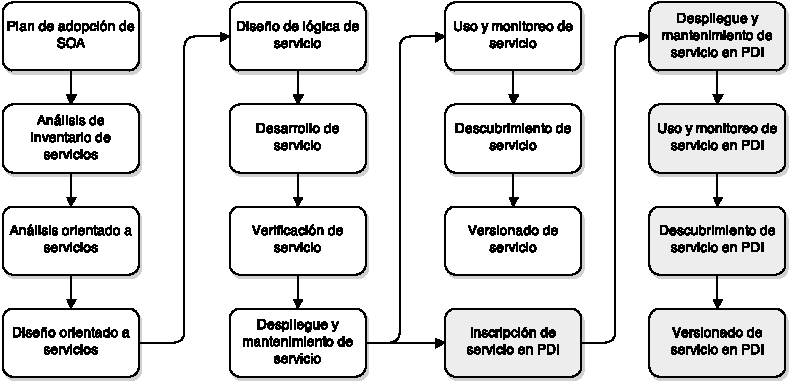
\includegraphics[width=\linewidth]{ciclo_de_vida_propuesta}
			    \caption{Ciclo de vida de proyecto y servicios propuesto}
			    \label{figura:ciclo_de_vida_propuesta}
			\end{figure}

		\subsection{Propuesta de gobernanza}
			Como se establece en la introducción, la gobernanza estará aplicada a las etapas posteriores a la puesta en producción en la infraestructura del organismo en cuestión:
			\begin{enumerate}
				\item Despliegue y mantenimiento
				\item Uso y monitoreo
				\item Descubrimiento
				\item Versionado y retiro
			\end{enumerate}

			\subsubsection{Despliegue y mantenimiento}
				En esta etapa se lleva a cabo la configuración del acceso al servicio por parte de los consumidores a través de la plataforma de interoperabilidad disponible en AGESIC.

				Esta es una segunda etapa de implantación ya que la primera ocurre sobre la infraestructura del organismo. En este caso, el objetivo es instalar la comunicación entre la PDI y el servicio desplegado del lado del organismo, lo que implica la aplicación de un patrón Proxy para intermediar en la comunicación con el servicio. Se deberán seguir las políticas ya existentes de seguridad y control de acceso a la plataforma, lo que implica la mantención del procedimiento y políticas de suscripción y publicación de servicios existentes.

				Para este procedimiento se contará con personal en el rol de desarrollador, quienes contarán con una especificación del servicio que les permitirá establecer la comunicación a través de la PDI. Esta especificación será obtenida a través del formulario de publicación de servicios, completado por los organismos al momento de publicar sus servicios en la PDI. La versión actual del mismo está disponible en.

				Luego de completar la etapa de despliegue, será necesario entrar en fase de verificación para asegurar el cumplimiento de los requisitos de configuración, así como también la calidad del servicio establecida en el acuerdo de nivel de servicio (siglas en Inglés, SLA). Hablaremos en detalle sobre calidad en la sección X de este informe. Los procesos de verificación llevados a cabo abarcarán a todos aquellos que aseguren una correcta comunicación entre la infraestructura de la plataforma de interoperabilidad y la del organismo proveedor del servicio, así como también el correcto funcionamiento de los controles de seguridad y acceso autorizado. Aquí entra en juego el rol de especialista en aseguramiento de la calidad. En esta sub-etapa no se verificará el funcionamiento en cuanto a la lógica del servicio en cuestión sino únicamente una comunicación exitosa; este tipo de verificación se asumirá completada por parte del organismo proveedor al momento de realizar el despliegue.

				El mantenimiento como se sugiere, implica una verificación periódica de los sistemas que mantienen al servicio disponible y especialmente, en cumplimiento con su SLA. AGESIC realizará las tareas de mantenimiento necesarias para mantener la comunicación entre la el proxy en la PDI y el servicio funcionando y respetando los niveles de servicio establecidos por contrato con los organismos consumidores. Será necesario monitorear atributos de calidad de los servicios con el fin de determinar las tareas necesarias. El encargado del mantenimiento será el personal disponible del área de desarrollo de AGESIC.

				Durante las tareas de mantenimiento, se tomará en cuenta la información provista por los consumidores en cuanto a horarios de uso del servicio, de modo de planificar la ejecución fuera de los horarios «pico» de utilización.

			\subsubsection{Uso y monitoreo}
				Durante el uso y monitoreo de los servicios, AGESIC se encargará de recolectar los valores de las mediciones correspondientes para asegurar la calidad y buen funcionamiento del servicio, así como también servir de retroalimentación para las actividades de mantenimiento y cobro por acceso.

				Periódicamente se realizarán actividades de revisión de funcionamiento sobre los servicios para determinar la necesidad de realizar ajustes sobre la configuración del acceso, independientemente de las revisiones de vitalidad que se realicen bajo la gobernanza del propio organismo sobre la lógica del servicio.

				Para realizar estas revisiones se tomarán en cuenta atributos de calidad que tengan impacto sobre la carga del servicio. Por ejemplo, un servicio que esté experimentando “picos” de uso periódicamente, deberá someter su configuración a revisión por parte del equipo de analistas de AGESIC para determinar la necesidad y viabilidad de un aumento de recursos para el proxy intermediario.

				Para hacer posible la detección de estas situaciones, se contará con un sistema de monitoreo sobre los servicios, el cual estará configurado en base a un modelo de calidad (abordado en la sección X). No se especifica en esta propuesta una forma de monitoreo particular; en base a la infraestructura existente, se sugiere la instalación de módulos de medición de atributos de calidad en la infraestructura de un Enterprise Service Bus (ESB).

			\subsubsection{Descubrimiento}
				Siguiendo el principio de \emph{Service Discoverability} (una ponderación sobre qué tan sencillo es encontrar un servicio), será necesario hacer que los servicios dispongan de suficientes meta-datos que permitan a un potencial usuario, descubrirlo y reutilizarlo en sus procesos de negocio, de manera de no solicitar la creación de nuevos servicios que cubran en todo o en parte lo que servicios ya existentes.

				Para facilitar el descubrimiento se establece una serie de meta-datos básicos de los que todos los servicios deben disponer. Esta información será desplegada en un registro central (central registry), gobernado por AGESIC. Este registro será independiente de los posibles registros gobernados por cada organismo, ya que contendrá sus propios meta-datos predefinidos y almacenados al momento de la publicación/migración.

				El acceso a este registro será público a través de la Internet. El sitio web se hará disponible a través de un servidor web gestionado por AGESIC. Se aplicará un criterio de confidencialidad sobre los meta-datos “sensibles”, de forma de no hacerlos disponibles a través del catálogo público, de existir.
				Algunos servicios podrán requerir ser marcados como privados, y por tanto sólo descubribles a en forma interna y con acceso autorizado. Esto deberá someterse a evaluación por parte del proveedor del servicio, en caso de que así se indique en la solicitud de publicación.

				Personal en el rol de custodio de servicios se encargaran de revisar los datos de los servicios publicados para asegurar la completitud y veracidad de los mismos. Un mismo custodio podrá estar encargado de más de un inventario de servicios, de ser necesario; no se establecen restricciones al respecto.

				El registro no permitirá la gestión del acceso al servicio a través de la web, sino que se continuará con el procedimiento actual de gestión de la publicación a través de formularios. Se sugiere con énfasis la implementación de un sistema electrónico independiente para la gestión de la publicación y solicitud de implementación de servicios.

				Ante situaciones de descubrimiento de servicios que resulten en solicitudes de modificaciones, las mismas serán transmitidas al organismo proveedor responsable y se pondrá en contacto al solicitante con dicho proveedor para negociar los cambios, los cuales, podrían resultar en una posterior migración de versión, situación descrita en la próxima sección.

				Una buena etapa de descubrimiento de servicios, requiere de la participación en la etapa del diseño orientado a servicio. Sin embargo, como hemos visto, AGESIC no participa de dicha etapa, por lo que la definición o modificación de meta-datos de uno o más servicios, puede requerir de contactar a los diseñadores responsables de cada uno.

				En la sección X introducimos una descripción de la implementación de un prototipo de registro central de servicios.

			\subsubsection{Versionado y retiro}
				Una nueva versión de un servicio será gestionada a partir de la solicitud por parte del organismo responsable. El procedimiento para la solicitud será similar al de la publicación, con el rellenado de un formulario especificando información relevante al cambio de versión. Esta actividad puede requerir de interacción entre responsables para determinar el procedimiento a seguir en cuanto a la configuración de la PDI y los cambios que potencialmente será necesario realizar para mantener el funcionamiento.

				Se aplicará la técnica de versionado desarrollada en la sección A DEFINIR.

				El retiro definitivo de servicios deberá ser planificado y anunciado cuanto antes a los organismos dependientes, de forma de permitirles establecer un curso de acción. Esto puede resultar difícil si el organismo proveedor omite el anuncio a AGESIC sobre la pre-determinación del retiro. Lo ideal será considerado que un servicio se encuentre en estado «deprecated» por un periodo no menor a 90 días, y esto sea anunciado con igual anticipación a los organismos dependientes. Pasado el periodo, el servicio (Proxy) será dado de baja de la PDI, así como también las configuraciones de seguridad y control de acceso establecidas para el mismo.

				Para determinar las dependencias, se utilizará un registro de consumidores de cada servicio, disponible desde el momento de cada suscripción.


	\section{Anexos}
		\subsection{Anexo I: Una breve descripción sobre las etapas del ciclo de vida que ocurren únicamente en los organismos}
			\label{sec:anexo1}
			El \emph{análisis de inventario de servicios} implica definir un grupo de entidades y procesos de negocio que permitan establecer una estructura básica para los servicios contenidos dentro del inventario (\emph{service blueprints}), de modo que estos no se superpongan entre sí y trabajen en conjunto de forma óptima para los procesos que abarca dicho inventario. El éxito de esta etapa requiere de conocimiento sobre el y/o los negocios de la organización.

			Un \emph{análisis orientado a servicio} es la primer etapa en la definición de servicios individuales. Esta etapa contribuye a los service blueprints y tiene como objetivo la identificación de distintos tipos de servicios dentro de el o los inventarios definidos.

			El \emph{diseño orientado a servicio} es un paso más hacia la definición de cada servicio; en esta etapa se definen los contratos de software que deberán cumplir los mismos. Estos son elaborados entre analistas de negocios y arquitectos.

			Una vez obtenido el contrato, se pasa a elaborar el \emph{diseño de la lógica de servicio} para su posterior \emph{desarrollo} y \emph{verificación}, los cuales requieren de arquitectos, analistas de negocios, desarrolladores y especialistas en aseguramiento de la calidad, roles que deben estar especializados en el área de negocio del organismo.


	\bibliographystyle{plain}
	\bibliography{proyecto_de_grado}
\end{document}